\documentclass[a4paper]{article}

\usepackage{graphicx}
\usepackage{amsmath,amssymb}
\usepackage{minted}
\usepackage{multirow}
\usepackage{float}
\usepackage{todonotes}
\usepackage{forest}
\usepackage{xstring}
\usepackage{xcolor}
\usepackage[most]{tcolorbox}
\usepackage{xparse}
\usepackage{natbib}

\usetikzlibrary{graphs,graphdrawing}
\usegdlibrary{layered}

% for external graphviz
\input{/home/donkarlo/Dropbox/repo/nd_language_ai_project/src/nd_language_ai/formal/computer/programming/tex/latex/code_clips/external_graphviz.tex}

% for tags
\input{/home/donkarlo/Dropbox/repo/nd_language_ai_project/src/nd_language_ai/formal/computer/programming/tex/latex/parts/control_sequence/kind/semtag/semtag.tex}

% for links
\input{/home/donkarlo/Dropbox/repo/nd_language_ai_project/src/nd_language_ai/formal/computer/programming/tex/latex/code_clips/seehere.tex}

\title{Transduction}
\date{}
\author{Mohammad Rahmani}

\begin{document}
    \maketitle
    In physiology, transduction is the translation of arriving stimulus into an action potential by a sensory receptor \seeherefooter{https://en.wikipedia.org/wiki/Transduction_(physiology)}.
    
    In this video the lecturer explains the simplest possible course of events signal in the form of a molcule evolves to a electric signal in the form of a receptor potential that may causes a spiking in the connected sensory neuron.
    \seeherefooter{https://www.youtube.com/watch?v=d7kitk-knjA}
    This following Figure is derived from the aformentioned video that shows the stages of sensory transduction
    \begin{figure}[H]
        \centering
        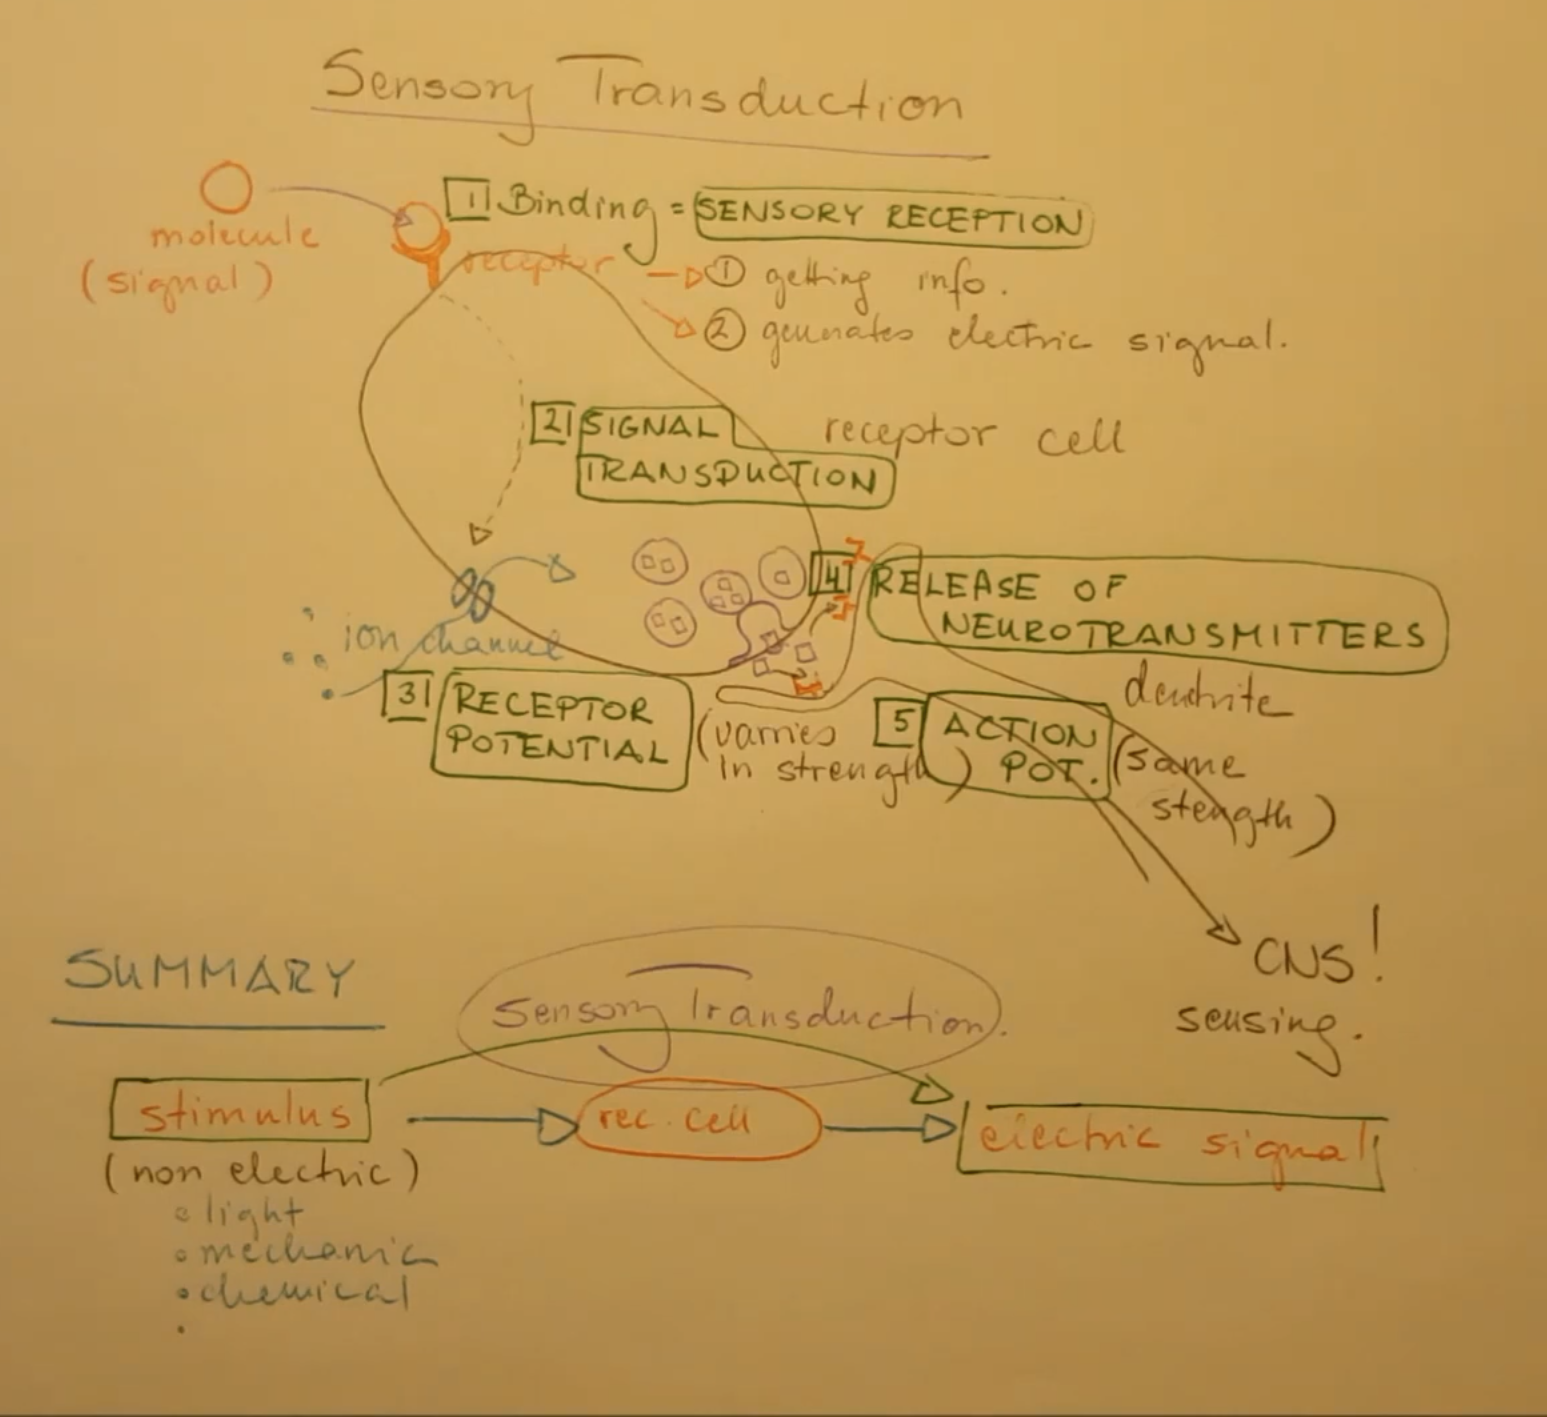
\includegraphics[width=0.9\textwidth]{transduction_stages.png}
    \end{figure}
    
%    \bibliographystyle{plainnat}
%    \bibliography{/home/donkarlo/Dropbox/repo/nd_shared_research/bibliography/bibliography.bib}
\end{document}